\documentclass[10pt]{article}
\usepackage{enumitem}
\usepackage{algorithm}
\usepackage[]{algorithmicx}
\usepackage{algpseudocode}
\usepackage{url}
\usepackage{tikz}
\usepackage{pgfplots}
\usepackage{amssymb} %Tools like \mathbb{, and mathfrak http://milde.users.sourceforge.net/LUCR/Math/mathpackages/amssymb-symbols.pdf
\usepackage{graphicx}
\usepackage{fancyhdr} %This is for HW, Documents, and stuff.
\usepackage{outlines}
\usepackage{courier}
\usepackage{verbatimbox}
\usepackage{changepage}   % for the adjustwidth environment
\usepackage{xcolor}
\usepackage{listings}
%\usepackage[caption=false]{subfig}
\usepackage{fancyvrb}
\usepackage{upquote}
\usepackage{multirow}
\usepackage{parskip} %to create whitespaces between paragraphs
\usepackage[cm]{fullpage} %Make pages take more space
\usepackage{float} %for figure placement.
\usepackage{verbatim} %for \begin{comment} \end{comment}    
\usepackage[mathscr]{euscript}
\usepackage{amsmath,amsthm,amssymb,latexsym,amsfonts}
%\usetikzlibrary{shadows}

%\usepackage{subcaption}
%\usepackage{etoolbox} %So many tools : https://www.ctan.org/pkg/etoolbox
%\usepackage{tabularx} %improves tables
%\renewcommand{\thesubsection}{Q.\arabic{subsection}}

\setcounter{secnumdepth}{4}

%For table spacing
\setlength{\tabcolsep}{5pt}
\renewcommand{\arraystretch}{1.2}


\title{Comparing graphs}
%\subtitle{}

\author {Adil Alsuhaim}
%\institute    {School of Computing \\ Clemson University}
\renewcommand{\familydefault}{\sfdefault}
\usepackage{gnuplot-lua-tikz}

\begin{document}
\maketitle
I this document, I illustrate the use of different graphics file formats. I use:
\begin{itemize}
  \item PNG : does not scale well. Should be used as a last resort.
  \item EPS : Scales very well, but the font is fixed in the image. Submission to conferences may ask you to use a supported font.
  \item Tikz: My preferred way. It scales well, and the font follows the document. 
\end{itemize}

\begin{figure}[H]
  \centering 
  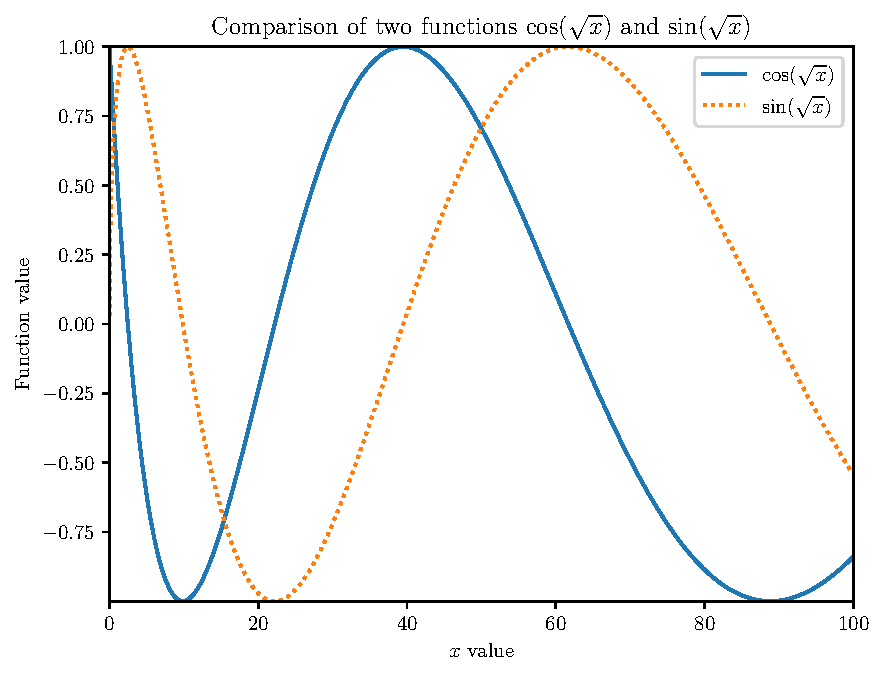
\includegraphics[width=0.75\columnwidth]{figures/FunctionCompare.pdf}
  \caption {Using \texttt{matplotlib} library generating a PDF}
\end{figure}

\begin{figure}[H]
  \centering 
  \resizebox{0.75\columnwidth}{!}{
    % This file was created with tikzplotlib v0.10.1.
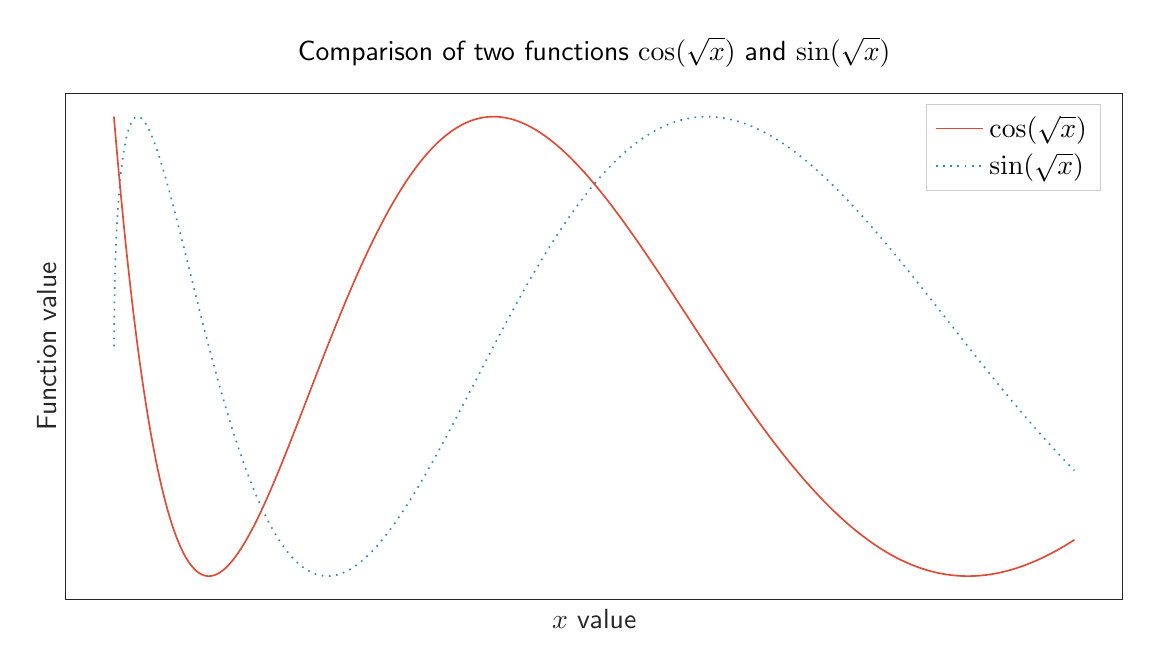
\begin{tikzpicture}

\definecolor{chocolate2267451}{RGB}{226,74,51}
\definecolor{darkslategray38}{RGB}{38,38,38}
\definecolor{lightgray204}{RGB}{204,204,204}
\definecolor{steelblue52138189}{RGB}{52,138,189}

\begin{axis}[
axis line style={darkslategray38},
height=8cm,
legend cell align={left},
legend style={fill opacity=0.8, draw opacity=1, text opacity=1, draw=lightgray204},
minor xtick={},
minor ytick={},
tick align=outside,
title={Comparison of two functions \(\displaystyle \cos (\sqrt{x})\) and \(\displaystyle \sin (\sqrt{x})\)},
width=15cm,
x grid style={lightgray204},
xlabel=\textcolor{darkslategray38}{\(\displaystyle x\) value},
xmajorticks=false,
xmin=-4.995, xmax=104.895,
xtick style={color=darkslategray38},
xtick={-20,0,20,40,60,80,100,120},
xticklabels={
  \(\displaystyle {\ensuremath{-}20}\),
  \(\displaystyle {0}\),
  \(\displaystyle {20}\),
  \(\displaystyle {40}\),
  \(\displaystyle {60}\),
  \(\displaystyle {80}\),
  \(\displaystyle {100}\),
  \(\displaystyle {120}\)
},
y grid style={lightgray204},
ylabel=\textcolor{darkslategray38}{Function value},
ymajorticks=false,
ymin=-1.0999997417313, ymax=1.09999998770149,
ytick style={color=darkslategray38},
ytick={-1.25,-1,-0.75,-0.5,-0.25,0,0.25,0.5,0.75,1,1.25},
yticklabels={
  \(\displaystyle {\ensuremath{-}1.25}\),
  \(\displaystyle {\ensuremath{-}1.00}\),
  \(\displaystyle {\ensuremath{-}0.75}\),
  \(\displaystyle {\ensuremath{-}0.50}\),
  \(\displaystyle {\ensuremath{-}0.25}\),
  \(\displaystyle {0.00}\),
  \(\displaystyle {0.25}\),
  \(\displaystyle {0.50}\),
  \(\displaystyle {0.75}\),
  \(\displaystyle {1.00}\),
  \(\displaystyle {1.25}\)
}
]
\addplot [semithick, chocolate2267451]
table {%
0 1
0.1 0.950415280255183
0.2 0.901655595150045
0.3 0.853712700224734
0.4 0.806578409885076
0.5 0.76024459707563
0.6 0.714703192954225
0.7 0.669946186567973
0.8 0.625965624530765
0.9 0.582753610702225
1 0.54030230586814
1.1 0.498603927422336
1.2 0.457650749050012
1.3 0.41743510041252
1.4 0.377949366833582
1.5 0.339185988986947
1.6 0.301137462585474
1.7 0.26379633807164
1.8 0.227155220309468
1.9 0.191206768277866
2 0.155943694765374
2.1 0.121358766066318
2.2 0.0874448016783473
2.3 0.0541946740013817
2.4 0.0216013080379287
2.5 -0.0103423189052092
2.6 -0.0416431775138572
2.7 -0.0723081867620183
2.8 -0.10234421420606
2.9 -0.131758076277542
3 -0.160556538574691
3.1 -0.18874631615252
3.2 -0.216334073811619
3.3 -0.243326426385591
3.4 -0.269729939027165
3.5 -0.295551127492978
3.6 -0.32079645842704
3.7 -0.345472349642868
3.8 -0.369585170404327
3.9 -0.393141241705146
4 -0.416146836547142
4.1 -0.438608180217149
4.2 -0.460531450562644
4.3 -0.481922778266099
4.4 -0.502788247118045
4.5 -0.523133894288856
4.6 -0.542965710599272
4.7 -0.562289640789645
4.8 -0.581111583787926
4.9 -0.599437392976401
5 -0.617272876457167
5.1 -0.634623797316366
5.2 -0.651495873887179
5.3 -0.667894780011574
5.4 -0.683826145300834
5.5 -0.699295555394849
5.6 -0.714308552220189
5.7 -0.728870634246955
5.8 -0.742987256744429
5.9 -0.756663832035498
6 -0.769905729749893
6.1 -0.782718277076217
6.2 -0.795106759012782
6.3 -0.807076418617265
6.4 -0.818632457255165
6.5 -0.829780034847093
6.6 -0.840524270114885
6.7 -0.850870240826538
6.8 -0.860822984039986
6.9 -0.870387496345718
7 -0.879568734108229
7.1 -0.888371613706332
7.2 -0.896801011772315
7.3 -0.904861765429954
7.4 -0.912558672531397
7.5 -0.919896491892905
7.6 -0.926879943529469
7.7 -0.933513708888301
7.8 -0.939802431081207
7.9 -0.945750715115839
8 -0.951363128125847
8.1 -0.956644199599912
8.2 -0.961598421609682
8.3 -0.966230249036615
8.4 -0.970544099797722
8.5 -0.974544355070221
8.6 -0.978235359515114
8.7 -0.981621421499676
8.8 -0.984706813318869
8.9 -0.98749577141569
9 -0.989992496600445
9.1 -0.992201154268967
9.2 -0.994125874619768
9.3 -0.99577075287014
9.4 -0.99713984947121
9.5 -0.998237190321942
9.6 -0.999066766982101
9.7 -0.99963253688418
9.8 -0.999938423544291
9.9 -0.999988316772033
10 -0.999786072879326
10.1 -0.999335514888231
10.2 -0.998640432737752
10.3 -0.997704583489625
10.4 -0.996531691533099
10.5 -0.995125448788709
10.6 -0.993489514911057
10.7 -0.991627517490587
10.8 -0.989543052254378
10.9 -0.987239683265939
11 -0.984720943124028
11.1 -0.981990333160483
11.2 -0.979051323637088
11.3 -0.975907353941456
11.4 -0.97256183278195
11.5 -0.969018138381637
11.6 -0.965279618671283
11.7 -0.961349591481394
11.8 -0.957231344733301
11.9 -0.952928136629296
12 -0.948443195841828
12.1 -0.943779721701755
12.2 -0.938940884385658
12.3 -0.933929825102225
12.4 -0.928749656277706
12.5 -0.923403461740436
12.6 -0.917894296904448
12.7 -0.912225188952158
12.8 -0.906399137016138
12.9 -0.900419112359985
13 -0.894288058558276
13.1 -0.888008891675624
13.2 -0.881584500444835
13.3 -0.875017746444167
13.4 -0.868311464273699
13.5 -0.861468461730817
13.6 -0.854491519984804
13.7 -0.847383393750563
13.8 -0.840146811461451
13.9 -0.83278447544125
14 -0.825299062075259
14.1 -0.817693221980527
14.2 -0.809969580175221
14.3 -0.802130736247134
14.4 -0.794179264521337
14.5 -0.786117714226986
14.6 -0.777948609663267
14.7 -0.769674450364515
14.8 -0.761297711264472
14.9 -0.752820842859723
15 -0.744246271372291
15.1 -0.735576398911398
15.2 -0.726813603634409
15.3 -0.71796023990694
15.4 -0.709018638462154
15.5 -0.69999110655924
15.6 -0.690879928141072
15.7 -0.681687363991065
15.8 -0.67241565188922
15.9 -0.663067006767368
16 -0.653643620863612
16.1 -0.644147663875975
16.2 -0.634581283115255
16.3 -0.624946603657082
16.4 -0.615245728493202
16.5 -0.605480738681968
16.6 -0.595653693498055
16.7 -0.585766630581392
16.8 -0.575821566085334
16.9 -0.565820494824049
17 -0.555765390419148
17.1 -0.545658205445546
17.2 -0.535500871576569
17.3 -0.525295299728292
17.4 -0.515043380203141
17.5 -0.504746982832723
17.6 -0.494407957119928
17.7 -0.484028132380274
17.8 -0.473609317882514
17.9 -0.463153302988507
18 -0.452661857292353
18.1 -0.442136730758795
18.2 -0.431579653860892
18.3 -0.420992337716973
18.4 -0.410376474226855
18.5 -0.399733736207354
18.6 -0.389065777527076
18.7 -0.378374233240492
18.8 -0.367660719721305
18.9 -0.356926834795111
19 -0.346174157871352
19.1 -0.335404250074574
19.2 -0.324618654374977
19.3 -0.313818895718282
19.4 -0.303006481154897
19.5 -0.292182899968395
19.6 -0.281349623803312
19.7 -0.270508106792252
19.8 -0.259659785682319
19.9 -0.24880607996087
20 -0.237948391980591
20.1 -0.227088107083905
20.2 -0.21622659372671
20.3 -0.205365203601447
20.4 -0.194505271759512
20.5 -0.183648116733006
20.6 -0.172795040655824
20.7 -0.161947329384095
20.8 -0.151106252615963
20.9 -0.140273064010729
21 -0.129449001307343
21.1 -0.118635286442245
21.2 -0.107833125666583
21.3 -0.0970437096627749
21.4 -0.08626821366045
21.5 -0.0755077975517497
21.6 -0.0647636060060045
21.7 -0.0540367685837813
21.8 -0.0433283998503053
21.9 -0.0326395994882709
22 -0.021971452410018
22.1 -0.0113250288691102
22.2 -0.000701384571284937
22.3 0.00989843921519486
22.4 0.0204734155498037
22.5 0.0310225317106185
22.6 0.0415447890857861
22.7 0.05203920306559
22.8 0.0625048029351174
22.9 0.0729406317675125
23 0.0833457463178296
23.1 0.0937192169174745
23.2 0.104060127369223
23.3 0.114367574842837
23.4 0.124640669771251
23.5 0.134878535747346
23.6 0.145080309421288
23.7 0.155245140398453
23.8 0.165372191137915
23.9 0.175460636851503
24 0.18550966540343
24.1 0.195518477210477
24.2 0.205486285142742
24.3 0.215412314424953
24.4 0.225295802538322
24.5 0.235135999122974
24.6 0.244932165880906
24.7 0.254683576479507
24.8 0.264389516455622
24.9 0.274049283120156
25 0.283662185463226
25.1 0.293227544059844
25.2 0.302744690976142
25.3 0.312212969676129
25.4 0.321631734928982
25.5 0.331000352716861
25.6 0.340318200143258
25.7 0.349584665341862
25.8 0.358799147385955
25.9 0.367961056198323
26 0.377069812461686
26.1 0.386124847529638
26.2 0.39512560333811
26.3 0.404071532317334
26.4 0.412962097304321
26.5 0.421796771455842
26.6 0.430575038161913
26.7 0.439296390959783
26.8 0.447960333448421
26.9 0.456566379203495
27 0.465114051692853
27.1 0.473602884192491
27.2 0.482032419703013
27.3 0.490402210866578
27.4 0.498711819884333
27.5 0.506960818434333
27.6 0.515148787589934
27.7 0.523275317738671
27.8 0.531340008501613
27.9 0.539342468653193
28 0.547282316041504
28.1 0.555159177509074
28.2 0.5629726888141
28.3 0.570722494552162
28.4 0.578408248078385
28.5 0.58602961143007
28.6 0.593586255249789
28.7 0.601077858708928
28.8 0.608504109431694
28.9 0.615864703419569
29 0.62315934497622
29.1 0.630387746632855
29.2 0.637549629074025
29.3 0.644644721063879
29.4 0.651672759372849
29.5 0.658633488704785
29.6 0.665526661624531
29.7 0.672352038485927
29.8 0.679109387360257
29.9 0.685798483965121
30 0.692419111593748
30.1 0.698971061044722
30.2 0.705454130552154
30.3 0.711868125716262
30.4 0.718212859434384
30.5 0.72448815183241
30.6 0.730693830196626
30.7 0.736829728905984
30.8 0.742895689364785
30.9 0.748891559935767
31 0.754817195873618
31.1 0.760672459258885
31.2 0.766457218932292
31.3 0.772171350429479
31.4 0.777814735916119
31.5 0.783387264123459
31.6 0.788888830284243
31.7 0.794319336069049
31.8 0.799678689523009
31.9 0.804966805002927
32 0.810183603114795
32.1 0.815329010651687
32.2 0.820402960532051
32.3 0.825405391738389
32.4 0.830336249256312
32.5 0.835195484013986
32.6 0.839983052821956
32.7 0.844698918313351
32.8 0.849343048884463
32.9 0.853915418635706
33 0.858416007312945
33.1 0.8628448002492
33.2 0.867201788306718
33.3 0.871486967819418
33.4 0.875700340535693
33.5 0.879841913561589
33.6 0.88391169930434
33.7 0.887909715416263
33.8 0.891835984739022
33.9 0.895690535248238
34 0.899473399998466
34.1 0.903184617068516
34.2 0.906824229507139
34.3 0.910392285279055
34.4 0.91388883721133
34.5 0.917313942940112
34.6 0.920667664857699
34.7 0.923950070059958
34.8 0.927161230294089
34.9 0.930301221906728
35 0.933370125792387
35.1 0.936368027342232
35.2 0.939295016393204
35.3 0.942151187177466
35.4 0.944936638272188
35.5 0.94765147254966
35.6 0.950295797127737
35.7 0.952869723320612
35.8 0.955373366589915
35.9 0.957806846496134
36 0.960170286650366
36.1 0.962463814666381
36.2 0.964687562113013
36.3 0.966841664466867
36.4 0.968926261065343
36.5 0.970941495059974
36.6 0.97288751337008
36.7 0.974764466636734
36.8 0.976572509177037
36.9 0.978311798938704
37 0.979982497454955
37.1 0.981584769799719
37.2 0.983118784543132
37.3 0.984584713707345
37.4 0.985982732722637
37.5 0.987313020383817
37.6 0.988575758806936
37.7 0.989771133386287
37.8 0.990899332751708
37.9 0.991960548726176
38 0.992954976283691
38.1 0.993882813507454
38.2 0.99474426154834
38.3 0.995539524583644
38.4 0.996268809776136
38.5 0.996932327233376
38.6 0.997530289967337
38.7 0.998062913854294
38.8 0.998530417595002
38.9 0.998933022675149
39 0.999270953326093
39.1 0.999544436485871
39.2 0.999753701760485
39.3 0.999898981385463
39.4 0.99998051018769
39.5 0.999998525547517
39.6 0.999953267361129
39.7 0.999844978003193
39.8 0.999673902289765
39.9 0.999440287441468
40 0.99914438304693
40.1 0.998786441026487
40.2 0.998366715596154
40.3 0.997885463231842
40.4 0.99734294263385
40.5 0.996739414691605
40.6 0.996075142448659
40.7 0.995350391067946
40.8 0.994565427797289
40.9 0.993720521935161
41 0.992815944796695
41.1 0.991851969679949
41.2 0.990828871832413
41.3 0.989746928417768
41.4 0.988606418482889
41.5 0.987407622925094
41.6 0.986150824459638
41.7 0.984836307587444
41.8 0.983464358563079
41.9 0.98203526536297
42 0.980549317653858
42.1 0.979006806761487
42.2 0.97740802563953
42.3 0.975753268838754
42.4 0.974042832476413
42.5 0.972277014205873
42.6 0.970456113186475
42.7 0.968580430053621
42.8 0.966650266889089
42.9 0.964665927191582
43 0.962627715847494
43.1 0.96053593910191
43.2 0.958390904529822
43.3 0.956192921007575
43.4 0.953942298684527
43.5 0.951639348954936
43.6 0.949284384430065
43.7 0.946877718910497
43.8 0.944419667358681
43.9 0.941910545871682
44 0.939350671654149
44.1 0.936740362991498
44.2 0.934079939223308
44.3 0.931369720716924
44.4 0.928610028841273
44.5 0.925801185940886
44.6 0.922943515310138
44.7 0.920037341167676
44.8 0.917082988631069
44.9 0.914080783691657
45 0.9110310531896
45.1 0.907934124789136
45.2 0.90479032695403
45.3 0.901599988923237
45.4 0.898363440686749
45.5 0.895081012961652
45.6 0.891753037168372
45.7 0.888379845407121
45.8 0.884961770434537
45.9 0.881499145640512
46 0.877992305025225
46.1 0.874441583176352
46.2 0.870847315246476
46.3 0.867209836930685
46.4 0.863529484444354
46.5 0.859806594501118
46.6 0.856041504291034
46.7 0.85223455145892
46.8 0.848386074082886
46.9 0.844496410653042
47 0.840565900050398
47.1 0.836594881525931
47.2 0.832583694679846
47.3 0.828532679441004
47.4 0.824442176046541
47.5 0.820312525021653
47.6 0.816144067159563
47.7 0.811937143501659
47.8 0.807692095317816
47.9 0.803409264086878
48 0.79908899147732
48.1 0.794731619328081
48.2 0.79033748962957
48.3 0.785906944504829
48.4 0.781440326190883
48.5 0.77693797702024
48.6 0.77240023940257
48.7 0.767827455806545
48.8 0.763219968741842
48.9 0.75857812074131
49 0.753902254343305
49.1 0.749192712074181
49.2 0.744449836430945
49.3 0.739673969864072
49.4 0.734865454760475
49.5 0.73002463342664
49.6 0.725151848071913
49.7 0.720247440791948
49.8 0.715311753552303
49.9 0.710345128172204
50 0.705347906308442
50.1 0.700320429439448
50.2 0.695263038849498
50.3 0.690176075613084
50.4 0.685059880579423
50.5 0.67991479435713
50.6 0.674741157299023
50.7 0.669539309487092
50.8 0.664309590717599
50.9 0.659052340486339
51 0.653767897974031
51.1 0.648456602031868
51.2 0.643118791167198
51.3 0.637754803529355
51.4 0.63236497689563
51.5 0.626949648657382
51.6 0.621509155806286
51.7 0.616043834920728
51.8 0.610554022152335
51.9 0.605040053212633
52 0.599502263359861
52.1 0.593940987385901
52.2 0.58835655960336
52.3 0.582749313832771
52.4 0.577119583389942
52.5 0.571467701073424
52.6 0.565793999152126
52.7 0.560098809353045
52.8 0.554382462849139
52.9 0.548645290247321
53 0.54288762157659
53.1 0.537109786276282
53.2 0.531312113184455
53.3 0.525494930526395
53.4 0.519658565903246
53.5 0.513803346280781
53.6 0.507929597978271
53.7 0.502037646657502
53.8 0.496127817311899
53.9 0.490200434255778
54 0.484255821113719
54.1 0.47829430081006
54.2 0.472316195558505
54.3 0.46632182685186
54.4 0.460311515451882
54.5 0.454285581379245
54.6 0.448244343903622
54.7 0.44218812153389
54.8 0.436117232008443
54.9 0.430031992285618
55 0.423932718534246
55.1 0.417819726124304
55.2 0.411693329617687
55.3 0.405553842759086
55.4 0.399401578466988
55.5 0.39323684882477
55.6 0.387059965071915
55.7 0.380871237595339
55.8 0.37467097592081
55.9 0.368459488704496
56 0.362237083724603
56.1 0.35600406787313
56.2 0.349760747147721
56.3 0.343507426643632
56.4 0.337244410545791
56.5 0.330972002120969
56.6 0.324690503710057
56.7 0.318400216720435
56.8 0.312101441618448
56.9 0.305794477921986
57 0.299479624193161
57.1 0.293157178031083
57.2 0.286827436064737
57.3 0.280490693945959
57.4 0.274147246342503
57.5 0.267797386931216
57.6 0.261441408391305
57.7 0.255079602397691
57.8 0.248712259614475
57.9 0.242339669688485
58 0.235962121242921
58.1 0.229579901871099
58.2 0.223193298130275
58.3 0.21680259553558
58.4 0.210408078554021
58.5 0.204010030598603
58.6 0.197608734022515
58.7 0.191204470113422
58.8 0.184797519087836
58.9 0.178388160085585
59 0.171976671164364
59.1 0.165563329294373
59.2 0.159148410353045
59.3 0.152732189119858
59.4 0.146314939271233
59.5 0.139896933375515
59.6 0.133478442888047
59.7 0.127059738146316
59.8 0.120641088365191
59.9 0.114222761632236
60 0.107805024903114
60.1 0.101388143997072
60.2 0.0949723835924935
60.3 0.0885580072225504
60.4 0.0821452772709213
60.5 0.0757344549675972
60.6 0.0693258003847598
60.7 0.0629195724327437
60.8 0.0565160288560722
60.9 0.0501154262295705
61 0.0437180199545611
61.1 0.0373240642551274
61.2 0.030933812174461
61.3 0.0245475155712744
61.4 0.0181654251162982
61.5 0.011787790288845
61.6 0.00541485937345369
61.7 -0.000953120543400611
61.8 -0.00731590357652201
61.9 -0.0136732450451316
62 -0.0200249014759406
62.1 -0.0263706306061502
62.2 -0.0327101913863819
62.3 -0.0390433439835333
62.4 -0.0453698497835731
62.5 -0.0516894713942578
62.6 -0.0580019726477868
62.7 -0.0643071186033866
62.8 -0.0706046755498258
62.9 -0.0768944110078703
63 -0.0831760937326625
63.1 -0.0894494937160395
63.2 -0.0957143821887905
63.3 -0.101970531622835
63.4 -0.108217715733356
63.5 -0.114455709480851
63.6 -0.120684289073127
63.7 -0.12690323196724
63.8 -0.133112316871356
63.9 -0.139311323746563
64 -0.145500033808614
64.1 -0.151678229529612
64.2 -0.157845694639636
64.3 -0.164002214128295
64.4 -0.170147574246247
64.5 -0.176281562506624
64.6 -0.182403967686431
64.7 -0.188514579827869
64.8 -0.194613190239594
64.9 -0.200699591497942
65 -0.206773577448069
65.1 -0.21283494320506
65.2 -0.218883485154957
65.3 -0.22491900095575
65.4 -0.230941289538307
65.5 -0.236950151107242
65.6 -0.242945387141737
65.7 -0.248926800396316
65.8 -0.254894194901537
65.9 -0.260847375964666
66 -0.266786150170276
66.1 -0.2727103253808
66.2 -0.278619710737034
66.3 -0.28451411665858
66.4 -0.290393354844251
66.5 -0.296257238272409
66.6 -0.302105581201272
66.7 -0.30793819916915
66.8 -0.313754908994646
66.9 -0.319555528776808
67 -0.325339877895217
67.1 -0.331107777010048
67.2 -0.336859048062067
67.3 -0.342593514272582
67.4 -0.34831100014336
67.5 -0.354011331456476
67.6 -0.359694335274136
67.7 -0.365359839938441
67.8 -0.371007675071108
67.9 -0.37663767157315
68 -0.382249661624505
68.1 -0.387843478683623
68.2 -0.393418957487018
68.3 -0.398975934048748
68.4 -0.404514245659893
68.5 -0.410033730887952
68.6 -0.415534229576221
68.7 -0.421015582843119
68.8 -0.426477633081471
68.9 -0.431920223957755
69 -0.437343200411302
69.1 -0.442746408653462
69.2 -0.448129696166727
69.3 -0.4534929117038
69.4 -0.458835905286654
69.5 -0.464158528205516
69.6 -0.469460633017846
69.7 -0.474742073547249
69.8 -0.480002704882365
69.9 -0.485242383375718
70 -0.490460966642525
70.1 -0.495658313559463
70.2 -0.500834284263411
70.3 -0.505988740150145
70.4 -0.511121543872998
70.5 -0.516232559341491
70.6 -0.521321651719919
70.7 -0.526388687425907
70.8 -0.531433534128928
70.9 -0.53645606074879
71 -0.541456137454083
71.1 -0.546433635660602
71.2 -0.55138842802972
71.3 -0.556320388466744
71.4 -0.561229392119225
71.5 -0.566115315375247
71.6 -0.570978035861673
71.7 -0.575817432442364
71.8 -0.580633385216361
71.9 -0.585425775516051
72 -0.590194485905275
72.1 -0.594939400177433
72.2 -0.599660403353535
72.3 -0.60435738168024
72.4 -0.609030222627851
72.5 -0.613678814888291
72.6 -0.618303048373039
72.7 -0.622902814211049
72.8 -0.627478004746625
72.9 -0.632028513537283
73 -0.636554235351573
73.1 -0.641055066166881
73.2 -0.645530903167196
73.3 -0.64998164474085
73.4 -0.654407190478245
73.5 -0.658807441169531
73.6 -0.663182298802271
73.7 -0.667531666559078
73.8 -0.671855448815228
73.9 -0.676153551136234
74 -0.680425880275419
74.1 -0.684672344171432
74.2 -0.688892851945773
74.3 -0.69308731390026
74.4 -0.697255641514504
74.5 -0.70139774744333
74.6 -0.705513545514197
74.7 -0.709602950724581
74.8 -0.71366587923934
74.9 -0.71770224838805
75 -0.721711976662331
75.1 -0.725694983713135
75.2 -0.729651190348024
75.3 -0.733580518528414
75.4 -0.73748289136681
75.5 -0.741358233124009
75.6 -0.745206469206287
75.7 -0.749027526162565
75.8 -0.75282133168155
75.9 -0.756587814588858
76 -0.76032690484412
76.1 -0.764038533538062
76.2 -0.767722632889566
76.3 -0.771379136242718
76.4 -0.775007978063826
76.5 -0.778609093938426
76.6 -0.782182420568273
76.7 -0.785727895768296
76.8 -0.789245458463558
76.9 -0.79273504868618
77 -0.796196607572253
77.1 -0.799630077358732
77.2 -0.803035401380316
77.3 -0.806412524066303
77.4 -0.809761390937437
77.5 -0.813081948602725
77.6 -0.816374144756255
77.7 -0.819637928173982
77.8 -0.822873248710506
77.9 -0.826080057295834
78 -0.829258305932118
78.1 -0.832407947690389
78.2 -0.83552893670727
78.3 -0.838621228181669
78.4 -0.841684778371469
78.5 -0.844719544590192
78.6 -0.847725485203654
78.7 -0.850702559626601
78.8 -0.853650728319344
78.9 -0.856569952784358
79 -0.859460195562889
79.1 -0.862321420231537
79.2 -0.865153591398825
79.3 -0.867956674701753
79.4 -0.870730636802355
79.5 -0.873475445384217
79.6 -0.876191069149011
79.7 -0.878877477812988
79.8 -0.881534642103488
79.9 -0.884162533755413
80 -0.886761125507702
80.1 -0.889330391099795
80.2 -0.891870305268076
80.3 -0.894380843742316
80.4 -0.896861983242097
80.5 -0.899313701473229
80.6 -0.901735977124154
80.7 -0.904128789862346
80.8 -0.906492120330689
80.9 -0.908825950143857
81 -0.911130261884677
81.1 -0.913405039100485
81.2 -0.915650266299473
81.3 -0.917865928947021
81.4 -0.920052013462029
81.5 -0.922208507213233
81.6 -0.924335398515517
81.7 -0.926432676626211
81.8 -0.928500331741384
81.9 -0.930538354992129
82 -0.932546738440841
82.1 -0.934525475077479
82.2 -0.936474558815835
82.3 -0.938393984489778
82.4 -0.940283747849504
82.5 -0.942143845557775
82.6 -0.943974275186146
82.7 -0.94577503521119
82.8 -0.947546125010719
82.9 -0.949287544859988
83 -0.950999295927902
83.1 -0.952681380273216
83.2 -0.954333800840722
83.3 -0.955956561457436
83.4 -0.957549666828778
83.5 -0.959113122534746
83.6 -0.960646935026084
83.7 -0.962151111620442
83.8 -0.96362566049854
83.9 -0.965070590700314
84 -0.966485912121063
84.1 -0.9678716355076
84.2 -0.969227772454382
84.3 -0.970554335399644
84.4 -0.971851337621533
84.5 -0.973118793234227
84.6 -0.974356717184061
84.7 -0.975565125245639
84.8 -0.97674403401795
84.9 -0.977893460920477
85 -0.979013424189301
85.1 -0.980103942873206
85.2 -0.981165036829774
85.3 -0.982196726721487
85.4 -0.983199034011813
85.5 -0.984171980961302
85.6 -0.98511559062367
85.7 -0.986029886841884
85.8 -0.986914894244246
85.9 -0.987770638240472
86 -0.988597145017768
86.1 -0.989394441536909
86.2 -0.990162555528312
86.3 -0.990901515488104
86.4 -0.991611350674198
86.5 -0.992292091102357
86.6 -0.992943767542265
86.7 -0.993566411513589
86.8 -0.994160055282046
86.9 -0.994724731855467
87 -0.995260474979858
87.1 -0.995767319135463
87.2 -0.996245299532824
87.3 -0.996694452108842
87.4 -0.997114813522837
87.5 -0.997506421152608
87.6 -0.997869313090491
87.7 -0.998203528139417
87.8 -0.998509105808978
87.9 -0.998786086311475
88 -0.999034510557989
88.1 -0.99925442015443
88.2 -0.999445857397607
88.3 -0.99960886527128
88.4 -0.999743487442228
88.5 -0.999849768256305
88.6 -0.999927752734508
88.7 -0.999977486569039
88.8 -0.999999016119366
88.9 -0.999992388408296
89 -0.999957651118037
89.1 -0.999894852586267
89.2 -0.999804041802206
89.3 -0.999685268402687
89.4 -0.999538582668229
89.5 -0.999364035519111
89.6 -0.99916167851145
89.7 -0.998931563833281
89.8 -0.998673744300635
89.9 -0.998388273353624
90 -0.998075205052527
90.1 -0.997734594073877
90.2 -0.997366495706548
90.3 -0.996970965847852
90.4 -0.996548060999635
90.5 -0.996097838264369
90.6 -0.995620355341259
90.7 -0.995115670522341
90.8 -0.994583842688597
90.9 -0.994024931306054
91 -0.993438996421906
91.1 -0.992826098660625
91.2 -0.992186299220084
91.3 -0.991519659867677
91.4 -0.990826242936446
91.5 -0.990106111321213
91.6 -0.989359328474712
91.7 -0.988585958403727
91.8 -0.987786065665232
91.9 -0.98695971536254
92 -0.986106973141448
92.1 -0.985227905186393
92.2 -0.98432257821661
92.3 -0.98339105948229
92.4 -0.982433416760751
92.5 -0.981449718352606
92.6 -0.980440033077938
92.7 -0.979404430272481
92.8 -0.978342979783802
92.9 -0.977255751967492
93 -0.976142817683359
93.1 -0.975004248291626
93.2 -0.973840115649136
93.3 -0.972650492105559
93.4 -0.971435450499607
93.5 -0.970195064155252
93.6 -0.968929406877948
93.7 -0.967638552950865
93.8 -0.966322577131121
93.9 -0.964981554646021
94 -0.963615561189304
94.1 -0.962224672917393
94.2 -0.960808966445655
94.3 -0.959368518844659
94.4 -0.957903407636447
94.5 -0.956413710790807
94.6 -0.954899506721556
94.7 -0.953360874282819
94.8 -0.951797892765329
94.9 -0.95021064189272
95 -0.948599201817834
95.1 -0.946963653119026
95.2 -0.94530407679649
95.3 -0.943620554268573
95.4 -0.941913167368108
95.5 -0.940181998338754
95.6 -0.93842712983133
95.7 -0.936648644900168
95.8 -0.934846626999473
95.9 -0.933021159979678
96 -0.931172328083815
96.1 -0.929300215943894
96.2 -0.927404908577281
96.3 -0.925486491383095
96.4 -0.923545050138592
96.5 -0.921580670995582
96.6 -0.91959344047683
96.7 -0.917583445472479
96.8 -0.915550773236471
96.9 -0.913495511382983
97 -0.911417747882863
97.1 -0.909317571060079
97.2 -0.907195069588171
97.3 -0.905050332486715
97.4 -0.902883449117789
97.5 -0.900694509182452
97.6 -0.898483602717227
97.7 -0.896250820090591
97.8 -0.893996251999479
97.9 -0.891719989465785
98 -0.889422123832881
98.1 -0.887102746762139
98.2 -0.884761950229459
98.3 -0.88239982652181
98.4 -0.880016468233777
98.5 -0.877611968264109
98.6 -0.87518641981229
98.7 -0.872739916375104
98.8 -0.870272551743214
98.9 -0.867784419997748
99 -0.865275615506896
99.1 -0.862746232922512
99.2 -0.860196367176725
99.3 -0.857626113478557
99.4 -0.855035567310552
99.5 -0.852424824425416
99.6 -0.849793980842657
99.7 -0.847143132845237
99.8 -0.844472376976237
99.9 -0.84178181003553
};
\addlegendentry{$\cos (\sqrt{x})$}
\addplot [semithick, steelblue52138189, dotted]
table {%
0 0
0.1 0.310983592907186
0.2 0.43245483895387
0.3 0.52074429951272
0.4 0.591127117215293
0.5 0.649636939080062
0.6 0.699427870463449
0.7 0.742409662587328
0.8 0.779850650384937
0.9 0.812648896642037
1 0.841470984807897
1.1 0.86682992770152
1.2 0.889132044127284
1.3 0.908706738691636
1.4 0.925826266699155
1.5 0.940719333741444
1.6 0.95358074048692
1.7 0.964578401178459
1.8 0.973858565648091
1.9 0.98154978058412
2 0.987765945992736
2.1 0.992608709360774
2.2 0.996169366453032
2.3 0.998530388776368
2.4 0.999766664522803
2.5 0.999946516789605
2.6 0.999132546645614
2.7 0.997382336983761
2.8 0.994749044643192
2.9 0.991281902051904
3 0.987026644990354
3.1 0.982025879566752
3.2 0.976319398817861
3.3 0.969944457287332
3.4 0.962936010331113
3.5 0.955326923643226
3.6 0.947148157502652
3.7 0.938428929451898
3.8 0.92919685848436
3.9 0.919478093306489
4 0.909297426825682
4.1 0.898678398675856
4.2 0.887643387314223
4.3 0.876213692992916
4.4 0.864409612718394
4.5 0.852250508152489
4.6 0.839754867275818
4.7 0.82694036052224
4.8 0.81382389199844
4.9 0.800421646322522
5 0.786749131547214
5.1 0.772821218575005
5.2 0.758652177422553
5.3 0.744255710648761
5.4 0.729644984223836
5.5 0.714832656084631
5.6 0.69983090259369
5.7 0.684651443095274
5.8 0.669305562740508
5.9 0.653804133735292
6 0.638157635148468
6.1 0.622376171403468
6.2 0.60646948956414
6.3 0.590446995514355
6.4 0.574317769121217
6.5 0.558090578462992
6.6 0.541773893195159
6.7 0.52537589712109
6.8 0.508904500027749
6.9 0.492367348841323
7 0.475771838152751
7.1 0.459125120158773
7.2 0.442434114060108
7.3 0.425705514954866
7.4 0.408945802262029
7.5 0.392161247707019
7.6 0.375357922898675
7.7 0.358541706524649
7.8 0.341718291190059
7.9 0.324893189922286
8 0.308071742363045
8.1 0.291259120667223
8.2 0.274460335126532
8.3 0.257680239534662
8.4 0.240923536309407
8.5 0.224194781386113
8.6 0.207498388895757
8.7 0.190838635640049
8.8 0.17421966537506
8.9 0.157645492914107
9 0.141120008059867
9.1 0.124646979375068
9.2 0.108230057800416
9.3 0.0918727801279254
9.4 0.0755785723372174
9.5 0.0593507528019202
9.6 0.0431925353728192
9.7 0.0271070323440086
9.8 0.0110972573078862
9.9 -0.00483387209549713
10 -0.0206835315295825
10.1 -0.0364489874080851
10.2 -0.0521275944328484
10.3 -0.0677167932184722
10.4 -0.083214107999671
10.5 -0.0986171444175446
10.6 -0.113923587381164
10.7 -0.129131199001076
10.8 -0.14423781659152
10.9 -0.15924135073833
11 -0.174139783429651
11.1 -0.188931166246768
11.2 -0.203613618612473
11.3 -0.218185326094549
11.4 -0.232644538762065
11.5 -0.246989569592296
11.6 -0.261218792926204
11.7 -0.275330642970515
11.8 -0.289323612344512
11.9 -0.303196250669791
12 -0.316947163201282
12.1 -0.330575009497933
12.2 -0.344078502131533
12.3 -0.357456405432225
12.4 -0.370707534269326
12.5 -0.383830752866128
12.6 -0.396824973647436
12.7 -0.409689156118636
12.8 -0.422422305775158
12.9 -0.435023473041234
13 -0.447491752236921
13.1 -0.45982628057238
13.2 -0.472026237168476
13.3 -0.484090842102773
13.4 -0.496019355480071
13.5 -0.507811076526635
13.6 -0.519465342707345
13.7 -0.530981528864968
13.8 -0.542359046380861
13.9 -0.553597342356376
14 -0.564695898814307
14.1 -0.575654231919739
14.2 -0.58647189121967
14.3 -0.597148458900826
14.4 -0.607683549065093
14.5 -0.618076807022023
14.6 -0.628327908597883
14.7 -0.638436559460752
14.8 -0.648402494461178
14.9 -0.658225476987921
15 -0.667905298338352
15.1 -0.677441777103051
15.2 -0.686834758564215
15.3 -0.696084114107462
15.4 -0.705189740646638
15.5 -0.714151560061287
15.6 -0.722969518646386
15.7 -0.731643586574032
15.8 -0.740173757366738
15.9 -0.748560047382014
16 -0.756802495307928
16.1 -0.764901161669352
16.2 -0.772856128344595
16.3 -0.780667498092164
16.4 -0.788335394087357
16.5 -0.795859959468459
16.6 -0.803241356892264
16.7 -0.8104797680987
16.8 -0.817575393484316
16.9 -0.824528451684397
17 -0.831339179163506
17.1 -0.838007829814225
17.2 -0.84453467456389
17.3 -0.850920000989143
17.4 -0.857164112938078
17.5 -0.863267330159819
17.6 -0.869229987941338
17.7 -0.875052436751343
17.8 -0.880735041891067
17.9 -0.886278183151789
18 -0.891682254478936
18.1 -0.896947663642604
18.2 -0.902074831914355
18.3 -0.907064193750144
18.4 -0.911916196479224
18.5 -0.91663129999892
18.6 -0.921209976475099
18.7 -0.92565271004825
18.8 -0.929959996545019
18.9 -0.934132343195087
19 -0.938170268353277
19.1 -0.942074301226773
19.2 -0.945844981607335
19.3 -0.949482859608407
19.4 -0.952988495407016
19.5 -0.956362458990345
19.6 -0.959605329906902
19.7 -0.962717697022171
19.8 -0.965700158278651
19.9 -0.968553320460214
20 -0.971277798960653
20.1 -0.973874217556379
20.2 -0.976343208183139
20.3 -0.978685410716711
20.4 -0.980901472757462
20.5 -0.982992049418723
20.6 -0.984957803118871
20.7 -0.986799403377079
20.8 -0.988517526612635
20.9 -0.990112855947766
21 -0.991586081013914
21.1 -0.992937897761369
21.2 -0.994169008272223
21.3 -0.995280120576558
21.4 -0.996271948471819
21.5 -0.997145211345311
21.6 -0.997900633999748
21.7 -0.99853894648182
21.8 -0.999060883913694
21.9 -0.999467186327418
22 -0.999758598502156
22.1 -0.999935869804216
22.2 -0.999999754029811
22.3 -0.999951009250505
22.4 -0.999790397661292
22.5 -0.999518685431275
22.6 -0.999136642556872
22.7 -0.998645042717531
22.8 -0.998044663133891
22.9 -0.997336284428355
23 -0.996520690488022
23.1 -0.995598668329953
23.2 -0.994571007968713
23.3 -0.99343850228616
23.4 -0.992201946903439
23.5 -0.99086214005514
23.6 -0.989419882465591
23.7 -0.987875977227235
23.8 -0.986231229681075
23.9 -0.984486447299131
24 -0.982642439568894
24.1 -0.980700017879727
24.2 -0.978659995411193
24.3 -0.97652318702327
24.4 -0.974290409148429
24.5 -0.971962479685528
24.6 -0.969540217895518
24.7 -0.967024444298905
24.8 -0.96441598057496
24.9 -0.96171564946263
25 -0.958924274663138
25.1 -0.95604268074424
25.2 -0.953071693046101
25.3 -0.950012137588785
25.4 -0.946864840981316
25.5 -0.943630630332289
25.6 -0.940310333162012
25.7 -0.936904777316147
25.8 -0.933414790880834
25.9 -0.929841202099269
26 -0.926184839289712
26.1 -0.922446530764908
26.2 -0.918627104752899
26.3 -0.914727389319201
26.4 -0.910748212290322
26.5 -0.90669040117861
26.6 -0.902554783108409
26.7 -0.898342184743491
26.8 -0.89405343221576
26.9 -0.889689351055193
27 -0.885250766121023
27.1 -0.880738501534112
27.2 -0.876153380610529
27.3 -0.871496225796287
27.4 -0.866767858603246
27.5 -0.861969099546145
27.6 -0.857100768080756
27.7 -0.852163682543145
27.8 -0.847158660090013
27.9 -0.842086516640113
28 -0.836948066816721
28.1 -0.831744123891145
28.2 -0.826475499727259
28.3 -0.821143004727043
28.4 -0.815747447777125
28.5 -0.810289636196293
28.6 -0.804770375683979
28.7 -0.799190470269691
28.8 -0.793550722263386
28.9 -0.787851932206761
29 -0.782094898825461
29.1 -0.776280418982182
29.2 -0.770409287630655
29.3 -0.764482297770506
29.4 -0.758500240402979
29.5 -0.752463904487493
29.6 -0.746374076899049
29.7 -0.740231542386447
29.8 -0.734037083531327
29.9 -0.727791480707999
30 -0.721495512044063
30.1 -0.715149953381817
30.2 -0.708755578240415
30.3 -0.702313157778791
30.4 -0.695823460759326
30.5 -0.689287253512249
30.6 -0.682705299900759
30.7 -0.676078361286866
30.8 -0.669407196497932
30.9 -0.662692561793908
31 -0.655935210835253
31.1 -0.649135894651529
31.2 -0.642295361610666
31.3 -0.635414357388873
31.4 -0.628493624941206
31.5 -0.621533904472767
31.6 -0.614535933410536
31.7 -0.607500446375824
31.8 -0.600428175157331
31.9 -0.593319848684821
32 -0.586176193003373
32.1 -0.57899793124824
32.2 -0.57178578362027
32.3 -0.564540467361904
32.4 -0.55726269673374
32.5 -0.549953182991647
32.6 -0.54261263436443
32.7 -0.535241756032033
32.8 -0.527841250104276
32.9 -0.520411815600114
33 -0.512954148427423
33.1 -0.505468941363283
33.2 -0.497956884034782
33.3 -0.490418662900299
33.4 -0.482854961231291
33.5 -0.47526645909456
33.6 -0.467653833334995
33.7 -0.460017757558783
33.8 -0.452358902117091
33.9 -0.444677934090196
34 -0.436975517272078
34.1 -0.429252312155447
34.2 -0.42150897591722
34.3 -0.413746162404415
34.4 -0.405964522120496
34.5 -0.398164702212118
34.6 -0.390347346456297
34.7 -0.382513095247992
34.8 -0.374662585588088
34.9 -0.366796451071774
35 -0.358915321877325
35.1 -0.351019824755265
35.2 -0.343110583017911
35.3 -0.335188216529298
35.4 -0.327253341695476
35.5 -0.319306571455179
35.6 -0.311348515270845
35.7 -0.303379779120001
35.8 -0.295400965487001
35.9 -0.287412673355109
36 -0.279415498198926
36.1 -0.271410031977152
36.2 -0.263396863125687
36.3 -0.255376576551058
36.4 -0.247349753624164
36.5 -0.239316972174358
36.6 -0.231278806483824
36.7 -0.223235827282278
36.8 -0.215188601741974
36.9 -0.207137693473007
37 -0.199083662518923
37.1 -0.191027065352614
37.2 -0.182968454872514
37.3 -0.174908380399068
37.4 -0.166847387671491
37.5 -0.158786018844808
37.6 -0.150724812487164
37.7 -0.142664303577402
37.8 -0.13460502350291
37.9 -0.126547500057738
38 -0.118492257440962
38.1 -0.11043981625531
38.2 -0.102390693506043
38.3 -0.0943454026000796
38.4 -0.086304453345365
38.5 -0.0782683519504886
38.6 -0.0702376010245294
38.7 -0.0622126995771446
38.8 -0.0541941430188857
38.9 -0.0461824231617434
39 -0.0381780282199168
39.1 -0.0301814428108075
39.2 -0.0221931479562263
39.3 -0.0142136210838183
39.4 -0.00624333602870204
39.5 0.00171723696468587
39.6 0.00966763124053495
39.7 0.0176073837294093
39.8 0.02553603494579
39.9 0.0334531289854242
40 0.041358213522474
40.1 0.0492508398064779
40.2 0.05713056265913
40.3 0.0649969404708553
40.4 0.0728495351972268
40.5 0.0806879123551752
40.6 0.088511641019043
40.7 0.0963202938164506
40.8 0.104113446923995
40.9 0.111890680062781
41 0.119651576493772
41.1 0.127395723012998
41.2 0.135122709946578
41.3 0.1428321311456
41.4 0.150523583980837
41.5 0.158196669337301
41.6 0.16585099160866
41.7 0.173486158691491
41.8 0.181101781979393
41.9 0.188697476356946
42 0.19627286019354
42.1 0.203827555337047
42.2 0.211361187107369
42.3 0.218873384289835
42.4 0.22636377912848
42.5 0.233832007319172
42.6 0.241277708002624
42.7 0.248700523757275
42.8 0.256100100592039
42.9 0.263476087938936
43 0.270828138645592
43.1 0.278155908967637
43.2 0.28545905856096
43.3 0.292737250473871
43.4 0.299990151139135
43.5 0.307217430365898
43.6 0.314418761331498
43.7 0.321593820573179
43.8 0.328742287979685
43.9 0.335863846782756
44 0.342958183548519
44.1 0.350024988168783
44.2 0.357063953852222
44.3 0.36407477711547
44.4 0.371057157774124
44.5 0.378010798933639
44.6 0.384935406980138
44.7 0.391830691571135
44.8 0.398696365626158
44.9 0.405532145317294
45 0.412337750059642
45.1 0.419112902501684
45.2 0.425857328515571
45.3 0.432570757187329
45.4 0.439252920806983
45.5 0.445903554858608
45.6 0.452522398010291
45.7 0.459109192104035
45.8 0.46566368214557
45.9 0.472185616294108
46 0.478674745852016
46.1 0.485130825254421
46.2 0.491553612058751
46.3 0.497942866934204
46.4 0.504298353651158
46.5 0.510619839070506
46.6 0.516907093132938
46.7 0.523159888848154
46.8 0.529378002284028
46.9 0.535561212555697
47 0.541709301814602
47.1 0.547822055237477
47.2 0.553899261015266
47.3 0.559940710342006
47.4 0.565946197403643
47.5 0.571915519366802
47.6 0.577848476367505
47.7 0.583744871499841
47.8 0.589604510804587
47.9 0.59542720325778
48 0.601212760759251
48.1 0.606960998121103
48.2 0.612671733056153
48.3 0.618344786166329
48.4 0.623979980931028
48.5 0.629577143695431
48.6 0.635136103658776
48.7 0.640656692862603
48.8 0.646138746178947
48.9 0.651582101298511
49 0.656986598718789
49.1 0.662352081732165
49.2 0.667678396413976
49.3 0.672965391610537
49.4 0.678212918927146
49.5 0.683420832716051
49.6 0.688588990064385
49.7 0.693717250782082
49.8 0.698805477389759
49.9 0.70385353510657
50 0.708861291838042
50.1 0.713828618163874
50.2 0.71875538732573
50.3 0.723641475214987
50.4 0.728486760360479
50.5 0.733291123916212
50.6 0.738054449649059
50.7 0.742776623926432
50.8 0.747457535703946
50.9 0.752097076513051
51 0.75669514044866
51.1 0.761251624156746
51.2 0.76576642682194
51.3 0.770239450155102
51.4 0.774670598380879
51.5 0.779059778225256
51.6 0.783406898903091
51.7 0.787711872105634
51.8 0.79197461198804
51.9 0.796195035156873
52 0.800373060657594
52.1 0.804508609962044
52.2 0.808601606955921
52.3 0.812651977926243
52.4 0.816659651548808
52.5 0.82062455887565
52.6 0.824546633322484
52.7 0.828425810656151
52.8 0.832262028982052
52.9 0.836055228731591
53 0.839805352649596
53.1 0.843512345781759
53.2 0.847176155462055
53.3 0.850796731300174
53.4 0.854374025168943
53.5 0.857907991191755
53.6 0.861398585729993
53.7 0.864845767370458
53.8 0.8682494969128
53.9 0.871609737356947
54 0.874926453890541
54.1 0.878199613876376
54.2 0.881429186839839
54.3 0.884615144456358
54.4 0.887757460538852
54.5 0.890856111025188
54.6 0.893911073965644
54.7 0.896922329510382
54.8 0.899889859896917
54.9 0.902813649437613
55 0.905693684507165
55.1 0.908529953530103
55.2 0.911322446968307
55.3 0.914071157308521
55.4 0.916776079049884
55.5 0.919437208691472
55.6 0.922054544719849
55.7 0.924628087596627
55.8 0.927157839746042
55.9 0.929643805542543
56 0.932085991298386
56.1 0.934484405251251
56.2 0.936839057551866
56.3 0.939149960251647
56.4 0.941417127290354
56.5 0.943640574483758
56.6 0.945820319511327
56.7 0.947956381903925
56.8 0.950048783031528
56.9 0.952097546090956
57 0.954102696093625
57.1 0.956064259853307
57.2 0.957982265973921
57.3 0.959856744837329
57.4 0.961687728591159
57.5 0.96347525113664
57.6 0.965219348116464
57.7 0.966920056902656
57.8 0.968577416584478
57.9 0.970191467956339
58 0.971762253505733
58.1 0.973289817401198
58.2 0.97477420548029
58.3 0.976215465237586
58.4 0.977613645812703
58.5 0.978968797978341
58.6 0.980280974128346
58.7 0.981550228265801
58.8 0.982776615991132
58.9 0.983960194490244
59 0.985101022522677
59.1 0.986199160409784
59.2 0.987254670022937
59.3 0.988267614771756
59.4 0.989238059592359
59.5 0.990166070935642
59.6 0.99105171675558
59.7 0.991895066497555
59.8 0.99269619108671
59.9 0.993455162916327
60 0.994172055836231
60.1 0.994846945141226
60.2 0.995479907559545
60.3 0.996071021241342
60.4 0.9966203657472
60.5 0.99712802203667
60.6 0.997594072456835
60.7 0.998018600730909
60.8 0.998401691946853
60.9 0.998743432546031
61 0.99904391031188
61.1 0.999303214358625
61.2 0.999521435120005
61.3 0.999698664338048
61.4 0.999834995051856
61.5 0.999930521586428
61.6 0.999985339541518
61.7 0.999999545780512
61.8 0.999973238419338
61.9 0.999906516815415
62 0.999799481556616
62.1 0.999652234450278
62.2 0.99946487851223
62.3 0.999237517955858
62.4 0.998970258181201
62.5 0.998663205764077
62.6 0.998316468445235
62.7 0.99793015511955
62.8 0.997504375825241
62.9 0.997039241733119
63 0.996534865135874
63.1 0.995991359437392
63.2 0.995408839142098
63.3 0.994787419844339
63.4 0.994127218217797
63.5 0.993428352004932
63.6 0.992690940006462
63.7 0.991915102070872
63.8 0.991100959083957
63.9 0.9902486329584
64 0.989358246623382
64.1 0.988429924014223
64.2 0.987463790062061
64.3 0.986459970683564
64.4 0.985418592770665
64.5 0.984339784180353
64.6 0.983223673724472
64.7 0.982070391159576
64.8 0.980880067176802
64.9 0.979652833391788
65 0.978388822334621
65.1 0.977088167439817
65.2 0.975751003036338
65.3 0.974377464337649
65.4 0.9729676874318
65.5 0.971521809271545
65.6 0.970039967664504
65.7 0.968522301263349
65.8 0.966968949556033
65.9 0.965380052856049
66 0.963755752292728
66.1 0.96209618980157
66.2 0.960401508114607
66.3 0.958671850750812
66.4 0.956907362006532
66.5 0.955108186945963
66.6 0.953274471391656
66.7 0.951406361915066
66.8 0.949504005827127
66.9 0.947567551168873
67 0.945597146702086
67.1 0.943592941899983
67.2 0.941555086937943
67.3 0.939483732684266
67.4 0.937379030690964
67.5 0.935241133184599
67.6 0.933070193057145
67.7 0.930866363856895
67.8 0.928629799779402
67.9 0.926360655658451
68 0.92405908695708
68.1 0.921725249758617
68.2 0.919359300757777
68.3 0.916961397251776
68.4 0.914531697131492
68.5 0.912070358872662
68.6 0.909577541527107
68.7 0.907053404714005
68.8 0.904498108611194
68.9 0.901911813946509
69 0.899294681989169
69.1 0.896646874541177
69.2 0.893968553928782
69.3 0.891259882993961
69.4 0.888521025085944
69.5 0.885752144052776
69.6 0.882953404232909
69.7 0.880124970446844
69.8 0.877267007988795
69.9 0.874379682618399
70 0.871463160552458
70.1 0.868517608456725
70.2 0.865543193437714
70.3 0.862540083034562
70.4 0.859508445210914
70.5 0.856448448346854
70.6 0.853360261230868
70.7 0.850244053051846
70.8 0.847099993391121
70.9 0.843928252214541
71 0.840728999864585
71.1 0.837502407052503
71.2 0.834248644850511
71.3 0.830967884684006
71.4 0.827660298323826
71.5 0.824326057878546
71.6 0.820965335786808
71.7 0.817578304809689
71.8 0.814165138023109
71.9 0.81072600881027
72 0.807261090854135
72.1 0.803770558129941
72.2 0.800254584897753
72.3 0.796713345695053
72.4 0.793147015329359
72.5 0.78955576887089
72.6 0.785939781645266
72.7 0.782299229226231
72.8 0.77863428742844
72.9 0.77494513230025
73 0.771231940116574
73.1 0.767494887371751
73.2 0.763734150772469
73.3 0.75994990723072
73.4 0.756142333856774
73.5 0.75231160795222
73.6 0.748457907003016
73.7 0.744581408672591
73.8 0.740682290794973
73.9 0.736760731367966
74 0.732816908546345
74.1 0.728851000635106
74.2 0.724863186082739
74.3 0.720853643474542
74.4 0.716822551525967
74.5 0.71277008907601
74.6 0.708696435080625
74.7 0.704601768606187
74.8 0.70048626882298
74.9 0.696350114998725
75 0.692193486492144
75.1 0.688016562746561
75.2 0.683819523283528
75.3 0.679602547696507
75.4 0.675365815644566
75.5 0.671109506846124
75.6 0.666833801072725
75.7 0.662538878142852
75.8 0.658224917915767
75.9 0.653892100285403
76 0.649540605174272
76.1 0.645170612527421
76.2 0.640782302306417
76.3 0.636375854483369
76.4 0.631951449034988
76.5 0.627509265936674
76.6 0.623049485156643
76.7 0.618572286650094
76.8 0.614077850353396
76.9 0.609566356178324
77 0.605037984006323
77.1 0.600492913682808
77.2 0.595931325011493
77.3 0.591353397748769
77.4 0.586759311598092
77.5 0.582149246204439
77.6 0.577523381148758
77.7 0.572881895942491
77.8 0.568224970022101
77.9 0.56355278274365
78 0.558865513377408
78.1 0.55416334110249
78.2 0.54944644500153
78.3 0.544715004055396
78.4 0.539969197137921
78.5 0.53520920301069
78.6 0.530435200317843
78.7 0.525647367580918
78.8 0.520845883193728
78.9 0.516030925417269
79 0.511202672374667
79.1 0.506361302046142
79.2 0.501506992264032
79.3 0.496639920707825
79.4 0.491760264899235
79.5 0.486868202197313
79.6 0.481963909793579
79.7 0.477047564707211
79.8 0.47211934378023
79.9 0.467179423672756
80 0.46222798085827
80.1 0.457265191618918
80.2 0.452291232040848
80.3 0.447306278009579
80.4 0.442310505205395
80.5 0.437304089098787
80.6 0.43228720494591
80.7 0.427260027784077
80.8 0.422222732427296
80.9 0.417175493461824
81 0.412118485241757
81.1 0.407051881884658
81.2 0.401975857267205
81.3 0.396890585020887
81.4 0.391796238527716
81.5 0.386692990915972
81.6 0.381581015055991
81.7 0.37646048355597
81.8 0.371331568757816
81.9 0.366194442733014
82 0.361049277278532
82.1 0.355896243912761
82.2 0.350735513871475
82.3 0.34556725810383
82.4 0.340391647268393
82.5 0.335208851729199
82.6 0.330019041551834
82.7 0.324822386499564
82.8 0.319619056029473
82.9 0.314409219288648
83 0.309193045110388
83.1 0.303970702010441
83.2 0.298742358183271
83.3 0.293508181498363
83.4 0.288268339496548
83.5 0.283022999386356
83.6 0.277772328040414
83.7 0.272516491991855
83.8 0.267255657430768
83.9 0.261989990200671
84 0.256719655795026
84.1 0.251444819353756
84.2 0.246165645659821
84.3 0.240882299135811
84.4 0.235594943840562
84.5 0.230303743465801
84.6 0.225008861332837
84.7 0.219710460389262
84.8 0.214408703205682
84.9 0.209103751972487
85 0.203795768496649
85.1 0.198484914198525
85.2 0.193171350108726
85.3 0.187855236864978
85.4 0.182536734709037
85.5 0.17721600348362
85.6 0.17189320262936
85.7 0.166568491181799
85.8 0.161242027768409
85.9 0.155913970605623
86 0.150584477495917
86.1 0.145253705824901
86.2 0.139921812558452
86.3 0.134588954239858
86.4 0.129255286987004
86.5 0.123920966489577
86.6 0.118586148006302
86.7 0.113250986362195
86.8 0.107915635945862
86.9 0.102580250706797
87 0.0972449841527424
87.1 0.091909989347039
87.2 0.086575418906024
87.3 0.0812414249964569
87.4 0.0759081593329531
87.5 0.0705757731754699
87.6 0.0652444173267919
87.7 0.0599142421300572
87.8 0.0545853974663157
87.9 0.0492580327520917
88 0.0439322969369928
88.1 0.0386083385013324
88.2 0.0332863054537811
88.3 0.0279663453290507
88.4 0.0226486051855831
88.5 0.0173332316032907
88.6 0.0120203706813027
88.7 0.00671016803574048
88.8 0.00140276879753048
88.9 -0.00390168238978655
89 -0.00920304137218515
89.1 -0.0145011644872921
89.2 -0.0197959085664777
89.3 -0.0250871309369342
89.4 -0.0303746894237239
89.5 -0.0356584423518091
89.6 -0.0409382485480463
89.7 -0.0462139673431751
89.8 -0.0514854585737627
89.9 -0.0567525825841375
90 -0.0620152002282949
90.1 -0.0672731728717818
90.2 -0.0725263623935548
90.3 -0.0777746311878123
90.4 -0.0830178421658115
90.5 -0.0882558587576511
90.6 -0.0934885449140474
90.7 -0.0987157651080659
90.8 -0.103937384336845
90.9 -0.109153268123293
91 -0.11436328251776
91.1 -0.119567294099694
91.2 -0.124765169979259
91.3 -0.12995677779895
91.4 -0.135141985735175
91.5 -0.140320662499808
91.6 -0.145492677341735
91.7 -0.15065790004837
91.8 -0.155816200947147
91.9 -0.160967450906991
92 -0.166111521339766
92.1 -0.171248284201716
92.2 -0.176377611994852
92.3 -0.181499377768354
92.4 -0.186613455119927
92.5 -0.191719718197138
92.6 -0.196818041698751
92.7 -0.201908300876007
92.8 -0.206990371533921
92.9 -0.212064130032524
93 -0.217129453288106
93.1 -0.222186218774434
93.2 -0.227234304523936
93.3 -0.232273589128883
93.4 -0.237303951742539
93.5 -0.242325272080292
93.6 -0.247337430420768
93.7 -0.252340307606921
93.8 -0.257333785047101
93.9 -0.262317744716113
94 -0.267292069156239
94.1 -0.272256641478248
94.2 -0.277211345362401
94.3 -0.282156065059402
94.4 -0.287090685391364
94.5 -0.292015091752735
94.6 -0.296929170111206
94.7 -0.301832807008615
94.8 -0.306725889561802
94.9 -0.311608305463485
95 -0.316479942983072
95.1 -0.321340690967498
95.2 -0.326190438841999
95.3 -0.33102907661091
95.4 -0.335856494858411
95.5 -0.340672584749268
95.6 -0.345477238029559
95.7 -0.350270347027377
95.8 -0.355051804653501
95.9 -0.359821504402081
96 -0.364579340351272
96.1 -0.369325207163866
96.2 -0.374059000087907
96.3 -0.378780614957272
96.4 -0.383489948192264
96.5 -0.388186896800152
96.6 -0.392871358375724
96.7 -0.397543231101794
96.8 -0.402202413749718
96.9 -0.406848805679878
97 -0.411482306842141
97.1 -0.416102817776326
97.2 -0.420710239612627
97.3 -0.425304474072032
97.4 -0.429885423466724
97.5 -0.434452990700469
97.6 -0.439007079268971
97.7 -0.443547593260231
97.8 -0.448074437354871
97.9 -0.452587516826459
98 -0.457086737541801
98.1 -0.461572005961225
98.2 -0.466043229138847
98.3 -0.470500314722827
98.4 -0.47494317095559
98.5 -0.479371706674055
98.6 -0.483785831309832
98.7 -0.488185454889406
98.8 -0.492570488034307
98.9 -0.496940841961266
99 -0.501296428482352
99.1 -0.505637160005091
99.2 -0.509962949532576
99.3 -0.514273710663559
99.4 -0.518569357592523
99.5 -0.522849805109745
99.6 -0.527114968601339
99.7 -0.53136476404929
99.8 -0.535599108031468
99.9 -0.539817917721621
};
\addlegendentry{$\sin (\sqrt{x})$}
\end{axis}

\end{tikzpicture}

  }
    
  \caption {Using \texttt{matplotlib} and \texttt{tikzplotlib} library}
\end{figure}

\begin{figure}[H]
  \centering 
  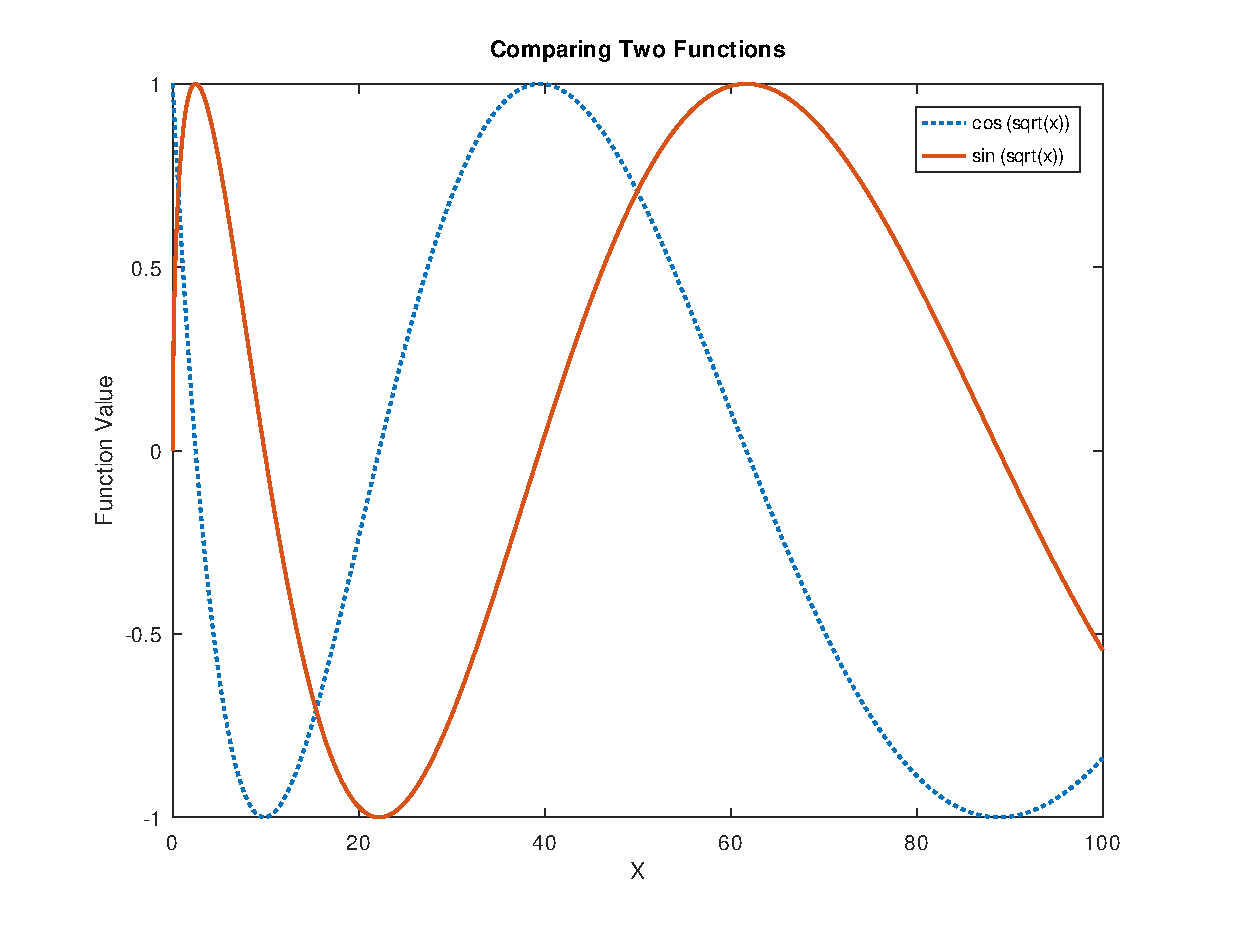
\includegraphics[width=0.75\columnwidth]{figures/OctaveEPS.eps}
  \caption {Using GNU Octave in EPS Format}
\end{figure}


\begin{figure}[H]
  \centering 
  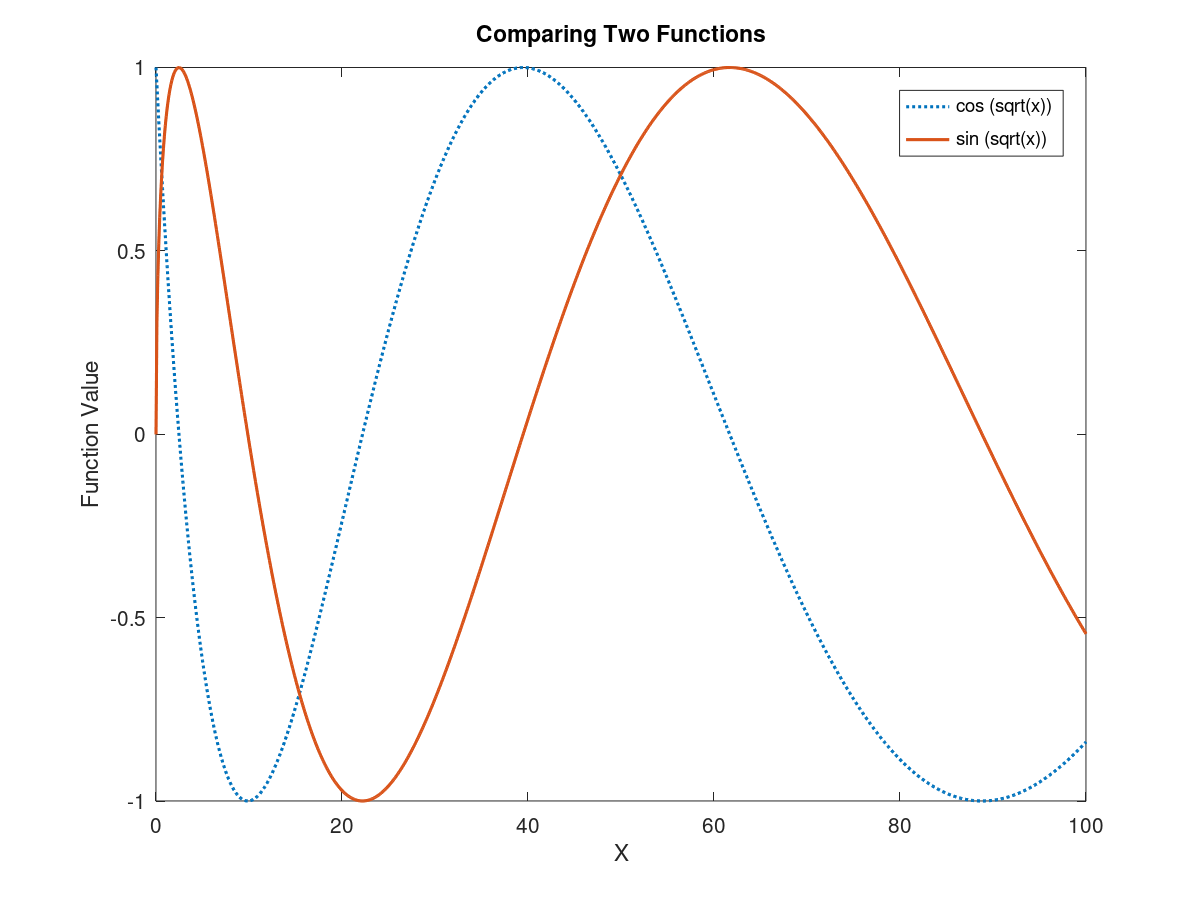
\includegraphics[width=0.75\columnwidth]{figures/OctavePNG.png}
  \caption {Using GNU Octave in PNG Format}
\end{figure}

\begin{figure}[H]
  \centering 
  \resizebox{0.75\columnwidth}{!}{
    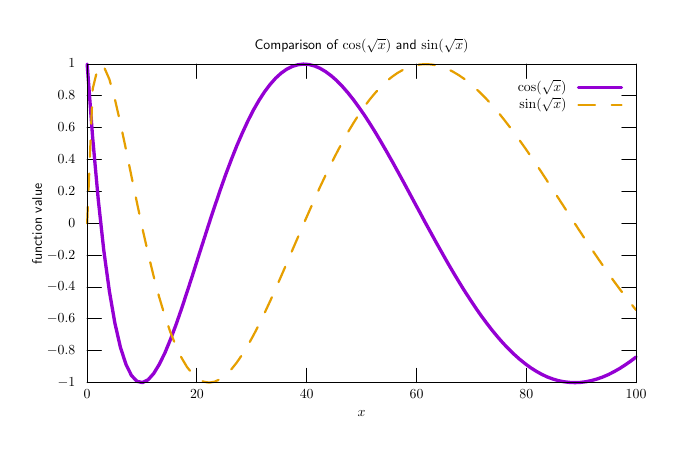
\begin{tikzpicture}[gnuplot]
  %% generated with GNUPLOT 5.2p2 (Lua 5.3; terminal rev. 99, script rev. 102)
  %% Thu 17 Sep 2020 09:36:52 PM EDT
  \tikzset{every node/.append style={scale=0.50}}
  \path (0.000,0.000) rectangle (8.000,5.000);
  \gpcolor{color=gp lt color border}
  \gpsetlinetype{gp lt border}
  \gpsetdashtype{gp dt solid}
  \gpsetlinewidth{1.00}
  \draw[gp path] (0.752,0.492)--(0.932,0.492);
  \draw[gp path] (7.723,0.492)--(7.543,0.492);
  \node[gp node right] at (0.660,0.492) {$-1$};
  \draw[gp path] (0.752,0.896)--(0.932,0.896);
  \draw[gp path] (7.723,0.896)--(7.543,0.896);
  \node[gp node right] at (0.660,0.896) {$-0.8$};
  \draw[gp path] (0.752,1.301)--(0.932,1.301);
  \draw[gp path] (7.723,1.301)--(7.543,1.301);
  \node[gp node right] at (0.660,1.301) {$-0.6$};
  \draw[gp path] (0.752,1.705)--(0.932,1.705);
  \draw[gp path] (7.723,1.705)--(7.543,1.705);
  \node[gp node right] at (0.660,1.705) {$-0.4$};
  \draw[gp path] (0.752,2.110)--(0.932,2.110);
  \draw[gp path] (7.723,2.110)--(7.543,2.110);
  \node[gp node right] at (0.660,2.110) {$-0.2$};
  \draw[gp path] (0.752,2.515)--(0.932,2.515);
  \draw[gp path] (7.723,2.515)--(7.543,2.515);
  \node[gp node right] at (0.660,2.515) {$0$};
  \draw[gp path] (0.752,2.919)--(0.932,2.919);
  \draw[gp path] (7.723,2.919)--(7.543,2.919);
  \node[gp node right] at (0.660,2.919) {$0.2$};
  \draw[gp path] (0.752,3.324)--(0.932,3.324);
  \draw[gp path] (7.723,3.324)--(7.543,3.324);
  \node[gp node right] at (0.660,3.324) {$0.4$};
  \draw[gp path] (0.752,3.728)--(0.932,3.728);
  \draw[gp path] (7.723,3.728)--(7.543,3.728);
  \node[gp node right] at (0.660,3.728) {$0.6$};
  \draw[gp path] (0.752,4.133)--(0.932,4.133);
  \draw[gp path] (7.723,4.133)--(7.543,4.133);
  \node[gp node right] at (0.660,4.133) {$0.8$};
  \draw[gp path] (0.752,4.537)--(0.932,4.537);
  \draw[gp path] (7.723,4.537)--(7.543,4.537);
  \node[gp node right] at (0.660,4.537) {$1$};
  \draw[gp path] (0.752,0.492)--(0.752,0.672);
  \draw[gp path] (0.752,4.537)--(0.752,4.357);
  \node[gp node center] at (0.752,0.338) {$0$};
  \draw[gp path] (2.146,0.492)--(2.146,0.672);
  \draw[gp path] (2.146,4.537)--(2.146,4.357);
  \node[gp node center] at (2.146,0.338) {$20$};
  \draw[gp path] (3.540,0.492)--(3.540,0.672);
  \draw[gp path] (3.540,4.537)--(3.540,4.357);
  \node[gp node center] at (3.540,0.338) {$40$};
  \draw[gp path] (4.935,0.492)--(4.935,0.672);
  \draw[gp path] (4.935,4.537)--(4.935,4.357);
  \node[gp node center] at (4.935,0.338) {$60$};
  \draw[gp path] (6.329,0.492)--(6.329,0.672);
  \draw[gp path] (6.329,4.537)--(6.329,4.357);
  \node[gp node center] at (6.329,0.338) {$80$};
  \draw[gp path] (7.723,0.492)--(7.723,0.672);
  \draw[gp path] (7.723,4.537)--(7.723,4.357);
  \node[gp node center] at (7.723,0.338) {$100$};
  \draw[gp path] (0.752,4.537)--(0.752,0.492)--(7.723,0.492)--(7.723,4.537)--cycle;
  \node[gp node center,rotate=-270] at (0.138,2.514) {function value};
  \node[gp node center] at (4.237,0.107) {{$ x $}};
  \node[gp node center] at (4.237,4.768) {Comparison of $ \cos (\sqrt{x}) $ and $ \sin (\sqrt{x}) $};
  \node[gp node right] at (6.899,4.244) {$ \cos (\sqrt{x}) $};
  \gpcolor{rgb color={0.580,0.000,0.827}}
  \gpsetlinewidth{3.00}
  \draw[gp path] (6.991,4.244)--(7.539,4.244);
  \draw[gp path] (0.752,4.537)--(0.822,3.599)--(0.893,2.816)--(0.963,2.172)--(1.034,1.654)%
    --(1.104,1.248)--(1.174,0.942)--(1.245,0.723)--(1.315,0.582)--(1.386,0.508)--(1.456,0.493)%
    --(1.527,0.529)--(1.597,0.608)--(1.667,0.723)--(1.738,0.867)--(1.808,1.036)--(1.879,1.224)%
    --(1.949,1.426)--(2.019,1.638)--(2.090,1.856)--(2.160,2.078)--(2.231,2.299)--(2.301,2.518)%
    --(2.372,2.732)--(2.442,2.939)--(2.512,3.137)--(2.583,3.325)--(2.653,3.502)--(2.724,3.666)%
    --(2.794,3.817)--(2.864,3.955)--(2.935,4.078)--(3.005,4.186)--(3.076,4.280)--(3.146,4.359)%
    --(3.216,4.423)--(3.287,4.473)--(3.357,4.508)--(3.428,4.529)--(3.498,4.537)--(3.569,4.532)%
    --(3.639,4.514)--(3.709,4.484)--(3.780,4.442)--(3.850,4.390)--(3.921,4.328)--(3.991,4.256)%
    --(4.061,4.176)--(4.132,4.087)--(4.202,3.991)--(4.273,3.889)--(4.343,3.781)--(4.414,3.667)%
    --(4.484,3.549)--(4.554,3.428)--(4.625,3.303)--(4.695,3.176)--(4.766,3.046)--(4.836,2.916)%
    --(4.906,2.785)--(4.977,2.654)--(5.047,2.523)--(5.118,2.394)--(5.188,2.266)--(5.259,2.140)%
    --(5.329,2.016)--(5.399,1.896)--(5.470,1.778)--(5.540,1.664)--(5.611,1.555)--(5.681,1.449)%
    --(5.751,1.348)--(5.822,1.252)--(5.892,1.161)--(5.963,1.075)--(6.033,0.995)--(6.103,0.921)%
    --(6.174,0.852)--(6.244,0.789)--(6.315,0.732)--(6.385,0.681)--(6.456,0.636)--(6.526,0.597)%
    --(6.596,0.564)--(6.667,0.538)--(6.737,0.517)--(6.808,0.503)--(6.878,0.495)--(6.948,0.492)%
    --(7.019,0.495)--(7.089,0.504)--(7.160,0.519)--(7.230,0.539)--(7.301,0.564)--(7.371,0.594)%
    --(7.441,0.630)--(7.512,0.670)--(7.582,0.715)--(7.653,0.764)--(7.723,0.817);
  \gpcolor{color=gp lt color border}
  \node[gp node right] at (6.899,4.019) {$ \sin (\sqrt{x}) $};
  \gpcolor{rgb color={0.902,0.624,0.000}}
  \gpsetdashtype{gp dt 2}
  \gpsetlinewidth{2.00}
  \draw[gp path] (6.991,4.019)--(7.539,4.019);
  \draw[gp path] (0.752,2.515)--(0.822,4.222)--(0.893,4.514)--(0.963,4.508)--(1.034,4.345)%
    --(1.104,4.092)--(1.174,3.786)--(1.245,3.453)--(1.315,3.110)--(1.386,2.770)--(1.456,2.440)%
    --(1.527,2.129)--(1.597,1.840)--(1.667,1.577)--(1.738,1.341)--(1.808,1.135)--(1.879,0.958)%
    --(1.949,0.810)--(2.019,0.692)--(2.090,0.602)--(2.160,0.540)--(2.231,0.504)--(2.301,0.492)%
    --(2.372,0.504)--(2.442,0.537)--(2.512,0.590)--(2.583,0.661)--(2.653,0.749)--(2.724,0.852)%
    --(2.794,0.967)--(2.864,1.094)--(2.935,1.231)--(3.005,1.376)--(3.076,1.528)--(3.146,1.685)%
    --(3.216,1.845)--(3.287,2.008)--(3.357,2.173)--(3.428,2.337)--(3.498,2.501)--(3.569,2.662)%
    --(3.639,2.821)--(3.709,2.976)--(3.780,3.126)--(3.850,3.271)--(3.921,3.410)--(3.991,3.543)%
    --(4.061,3.668)--(4.132,3.786)--(4.202,3.896)--(4.273,3.998)--(4.343,4.091)--(4.414,4.176)%
    --(4.484,4.252)--(4.554,4.319)--(4.625,4.377)--(4.695,4.426)--(4.766,4.466)--(4.836,4.497)%
    --(4.906,4.519)--(4.977,4.532)--(5.047,4.537)--(5.118,4.533)--(5.188,4.522)--(5.259,4.502)%
    --(5.329,4.475)--(5.399,4.440)--(5.470,4.398)--(5.540,4.350)--(5.611,4.295)--(5.681,4.234)%
    --(5.751,4.167)--(5.822,4.095)--(5.892,4.017)--(5.963,3.936)--(6.033,3.849)--(6.103,3.759)%
    --(6.174,3.666)--(6.244,3.569)--(6.315,3.470)--(6.385,3.368)--(6.456,3.264)--(6.526,3.158)%
    --(6.596,3.051)--(6.667,2.943)--(6.737,2.834)--(6.808,2.725)--(6.878,2.616)--(6.948,2.508)%
    --(7.019,2.400)--(7.089,2.293)--(7.160,2.187)--(7.230,2.083)--(7.301,1.980)--(7.371,1.879)%
    --(7.441,1.781)--(7.512,1.685)--(7.582,1.592)--(7.653,1.502)--(7.723,1.414);
  \gpcolor{color=gp lt color border}
  \gpsetdashtype{gp dt solid}
  \gpsetlinewidth{1.00}
  \draw[gp path] (0.752,4.537)--(0.752,0.492)--(7.723,0.492)--(7.723,4.537)--cycle;
  %% coordinates of the plot area
  \gpdefrectangularnode{gp plot 1}{\pgfpoint{0.752cm}{0.492cm}}{\pgfpoint{7.723cm}{4.537cm}}
  \end{tikzpicture}
  }
  \caption {Using \texttt{gnuplot} generated \texttt{tikzpicture} library}
\end{figure}

\begin{figure}[H]
  \centering 
  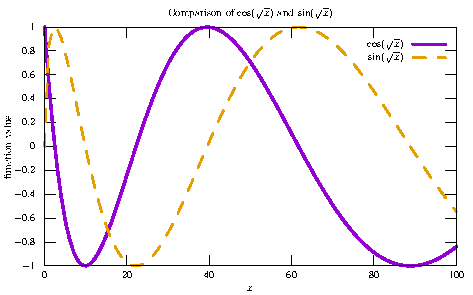
\includegraphics[width=0.75\columnwidth]{figures/GnuPlotPDF.pdf}
  \caption {Using \texttt{gnuplot} to generate a \LaTeX PDF}
\end{figure}

\begin{figure}[H]
  \centering 
  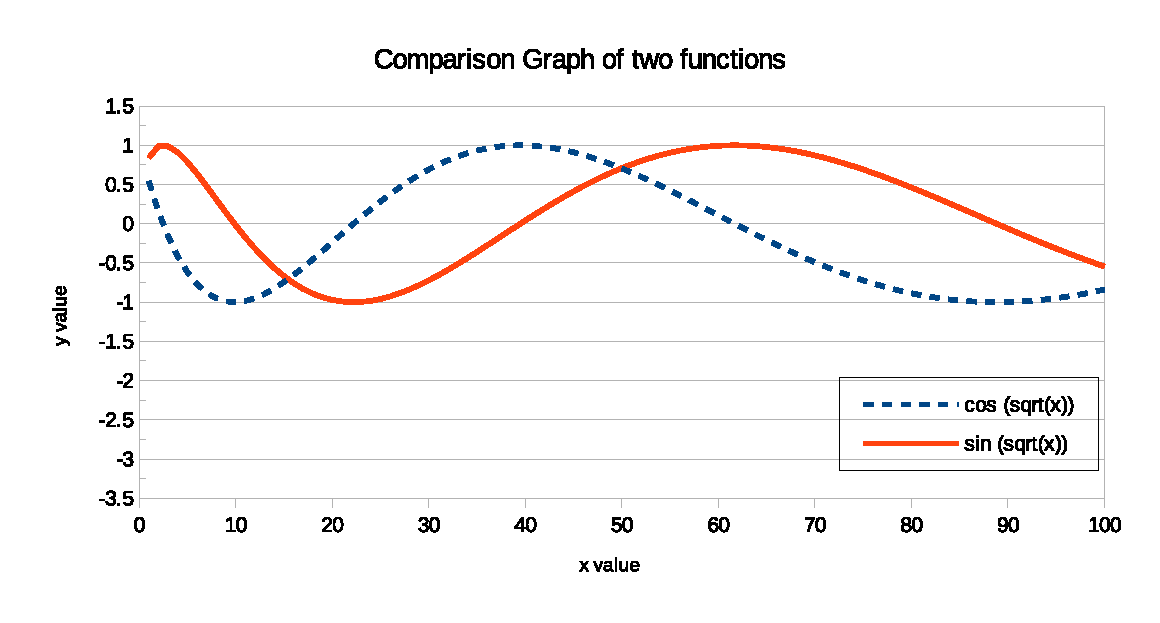
\includegraphics[width=0.75\columnwidth]{figures/LibreEPS.eps}
  \caption {Using LibreOffice in EPS Format}
\end{figure}


\begin{figure}[H]
  \centering 
  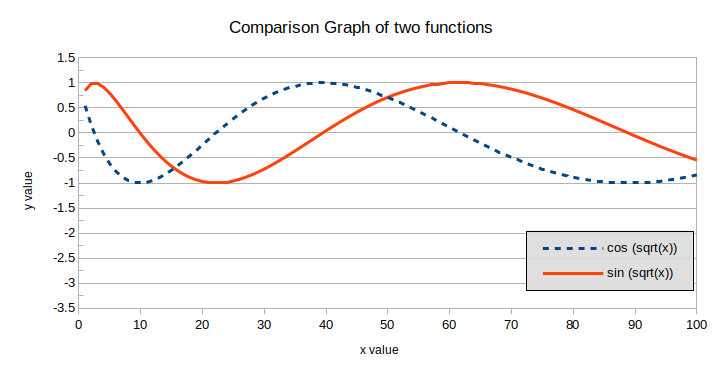
\includegraphics[width=0.75\columnwidth]{figures/LibrePNG.png}
  \caption {Using LibreOffice in PNG Format}
\end{figure}

\end{document}